% Apex user guide. Build with docs/user-guide/latex/build.sh (pdflatex, two
% passes). Written in British English. The layout is deliberately
% ADHD-friendly: every chapter opens with a one-box summary, sections are
% short, actions are bold, keys are boxed, and each chapter stands on its own
% so you can read in any order and stop at any point.
\documentclass[11pt,a4paper,oneside]{report}

\usepackage[utf8]{inputenc}
\usepackage[T1]{fontenc}
\usepackage{lmodern}
\usepackage[british]{babel}
\usepackage[margin=24mm,top=22mm,bottom=24mm]{geometry}
\usepackage{microtype}
\usepackage{xcolor}
\usepackage{graphicx}
\usepackage{booktabs}
\usepackage{tabularx}
\usepackage{longtable}
\usepackage{enumitem}
\usepackage{titlesec}
\usepackage{fancyhdr}
\usepackage{tcolorbox}
\usepackage{fancyvrb}
\usepackage[hidelinks,bookmarks=true,bookmarksopen=true,pdftitle={Apex User Guide},pdfauthor={Apex}]{hyperref}

% ---------------------------------------------------------------------------
% Colours and boxes
% ---------------------------------------------------------------------------
\definecolor{apexblue}{HTML}{2F6DB5}
\definecolor{apexink}{HTML}{23262E}
\definecolor{apexmist}{HTML}{EEF3FA}
\definecolor{apexsage}{HTML}{E9F5EC}
\definecolor{apexamber}{HTML}{FFF4DD}
\definecolor{apexrose}{HTML}{FBE9EA}
\definecolor{keybg}{HTML}{F3F4F6}
\definecolor{keyline}{HTML}{B8BCC6}

% "In a nutshell" summary at the top of every chapter: the one box to read
% if you read nothing else.
\newtcolorbox{nutshell}{colback=apexmist,colframe=apexblue,boxrule=0.8pt,
  arc=2pt,left=6pt,right=6pt,top=5pt,bottom=5pt,
  title=\textbf{In a nutshell},fonttitle=\small,coltitle=white}
% A tiny task to try straight away. Doing beats reading.
\newtcolorbox{tryit}{colback=apexsage,colframe=green!40!black,boxrule=0.6pt,
  arc=2pt,left=6pt,right=6pt,top=4pt,bottom=4pt,
  title=\textbf{Try it now (two minutes)},fonttitle=\small,coltitle=white}
% Something that bites if you miss it.
\newtcolorbox{watchout}{colback=apexamber,colframe=orange!70!black,boxrule=0.6pt,
  arc=2pt,left=6pt,right=6pt,top=4pt,bottom=4pt,
  title=\textbf{Watch out},fonttitle=\small,coltitle=white}
% Safety and privacy notes.
\newtcolorbox{safenote}{colback=apexrose,colframe=red!55!black,boxrule=0.6pt,
  arc=2pt,left=6pt,right=6pt,top=4pt,bottom=4pt,
  title=\textbf{Your data},fonttitle=\small,coltitle=white}

% A keyboard key: \key{Ctrl+P}. Boxed so it stands out when scanning.
\newcommand{\key}[1]{\fcolorbox{keyline}{keybg}{\footnotesize\texttt{#1}}}
% A menu path: \menu{File > Open Folder}.
\newcommand{\menu}[1]{\textbf{#1}}
% A setting key.
\newcommand{\setting}[1]{\texttt{#1}}

\titleformat{\chapter}[display]{\normalfont\huge\bfseries\color{apexblue}}{\chaptertitlename\ \thechapter}{8pt}{\Huge}
\titlespacing*{\chapter}{0pt}{0pt}{18pt}
\titleformat{\section}{\normalfont\Large\bfseries\color{apexink}}{\thesection}{1em}{}
\titleformat{\subsection}{\normalfont\large\bfseries\color{apexink}}{\thesubsection}{1em}{}

\setlist{nosep,itemsep=3pt,leftmargin=*}
\setlength{\parskip}{5pt}
\setlength{\parindent}{0pt}
% Long typewriter names (paths, server names) cannot hyphenate; let lines
% stretch a little rather than overflow the margin.
\setlength{\emergencystretch}{3em}
\renewcommand{\arraystretch}{1.25}

\pagestyle{fancy}
\fancyhf{}
\fancyhead[L]{\small\color{gray}Apex User Guide}
\fancyhead[R]{\small\color{gray}\nouppercase{\leftmark}}
\fancyfoot[C]{\small\thepage}
\renewcommand{\headrulewidth}{0.3pt}

\fvset{fontsize=\small,frame=lines,framesep=3pt,rulecolor=\color{keyline}}

\graphicspath{{../../screenshots/}}

\begin{document}

% ---------------------------------------------------------------------------
\begin{titlepage}
\centering
\vspace*{30mm}
{\Huge\bfseries\color{apexblue}Apex\par}
\vspace{4mm}
{\LARGE User Guide\par}
\vspace{6mm}
{\large Version 0.0.1 \par}
\vspace{14mm}
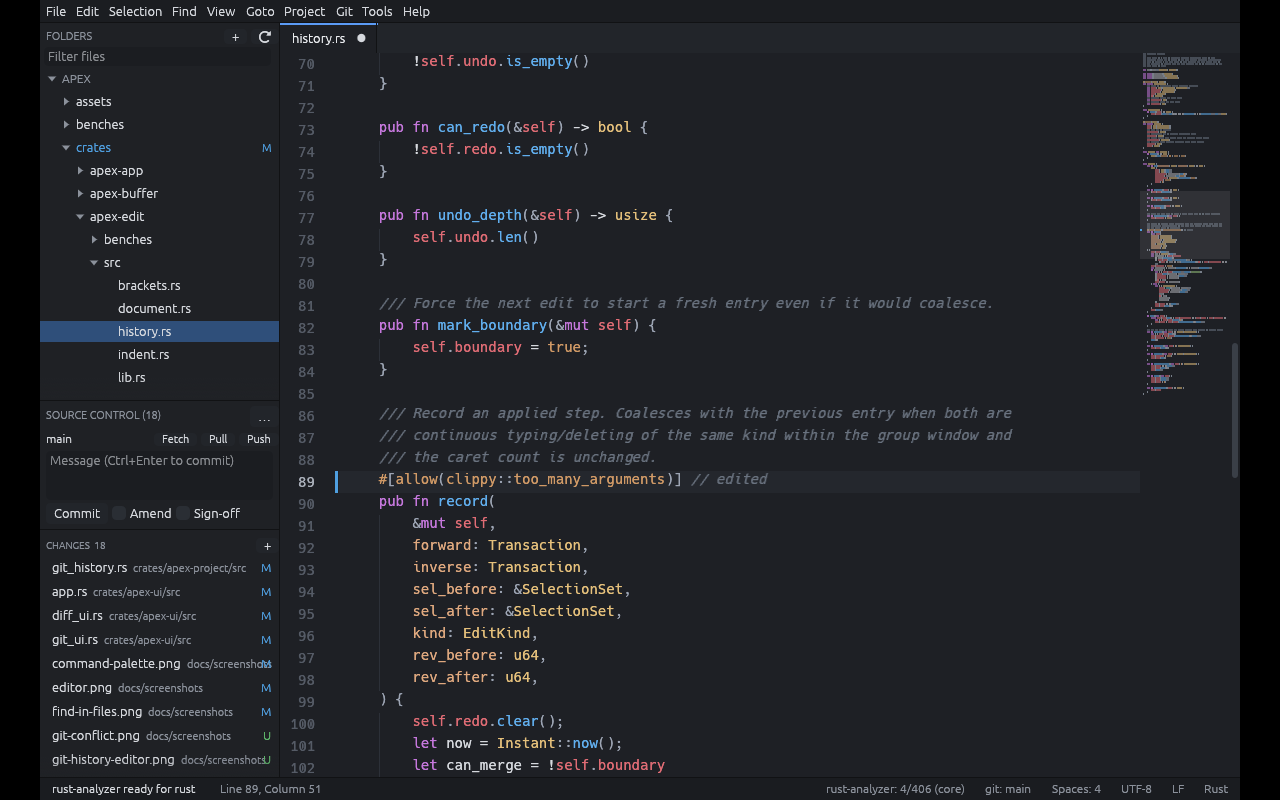
\includegraphics[width=0.85\textwidth]{editor.png}
\vspace{12mm}

\begin{minipage}{0.8\textwidth}
\begin{nutshell}
Apex is a fast, native text editor for Linux, macOS and Windows. It starts
instantly, edits with many cursors at once, finds anything in a project in
a keystroke, and understands Git. There are no plugins, no accounts and no
telemetry: everything works offline.
\end{nutshell}
\end{minipage}

\vfill
{\small Licensed under the GNU AGPL v3.0 or later.\par}
\end{titlepage}

% ---------------------------------------------------------------------------
\chapter*{How to use this guide}
\addcontentsline{toc}{chapter}{How to use this guide}

\begin{nutshell}
You do not need to read this in order. Every chapter starts with a box like
this one that says what the chapter is for. Read the box; if it is what you
need, carry on; if not, skip the chapter.
\end{nutshell}

\begin{itemize}
\item \textbf{Boxed keys} such as \key{Ctrl+P} are things to press.
\item \textbf{Bold text} such as \menu{File > Open Folder} is a menu path or a
  button to click.
\item \texttt{Typewriter text} is something to type, or a file name.
\item Green \textbf{Try it now} boxes are two-minute exercises. Doing one
  beats reading a page.
\item Amber \textbf{Watch out} boxes mark the things that catch people out.
\item Red \textbf{Your data} boxes say what Apex does, and does not do, with
  your files and credentials.
\end{itemize}

Shortcuts are written for Linux and Windows. On macOS read \key{Ctrl} as
\key{Cmd} unless the text says otherwise. \menu{Tools > Keyboard Shortcuts}
(\key{Ctrl+K Ctrl+S}) lists every binding for your platform, and the command
palette shows the shortcut next to each command.

\section*{The one-page cheat sheet}

\begin{tabularx}{\textwidth}{l X}
\toprule
\textbf{Keys} & \textbf{What happens} \\
\midrule
\key{Ctrl+P} & Goto Anything: files, \texttt{:line}, \texttt{@symbol}, \texttt{\#project symbol}, \texttt{>command} \\
\key{Ctrl+Shift+P} & Command palette: every command, with its shortcut \\
\key{Ctrl+O} / \key{Ctrl+Shift+O} & Open a file / open a folder \\
\key{Ctrl+S} & Save (atomic: a half-written file never replaces yours) \\
\key{Ctrl+D} & Select the word, then add the next occurrence each press \\
\key{Ctrl+Shift+L} & One cursor per selected line \\
\key{Ctrl+F} / \key{Ctrl+H} & Find / replace in the file \\
\key{Ctrl+Shift+F} & Find in files across the project \\
\key{Ctrl+B} & Run the build task \\
\key{Ctrl+K Ctrl+G} & Git blame on or off \\
\key{Ctrl+\textbackslash} & Split the pane \\
\key{F11} / \key{Shift+F11} & Fullscreen / distraction-free \\
\key{Escape} & Back to one cursor, close the bar, leave the mode \\
\bottomrule
\end{tabularx}

\tableofcontents

% ===========================================================================
\chapter{Getting started}

\begin{nutshell}
Install Apex, open a folder, and learn the shape of the window. Ten minutes.
\end{nutshell}

\section{Installing}

\begin{description}[style=nextline]
\item[Linux] Unpack \texttt{apex-<version>-linux-<arch>.tar.gz} and run
  \texttt{./install.sh} (installs to \texttt{\textasciitilde/.local}; prefix
  with \texttt{PREFIX=/usr/local sudo} for all users). Or install the
  \texttt{.deb} with \texttt{sudo apt install ./apex\_<version>\_amd64.deb}.
  The AppImage runs from anywhere after \texttt{chmod +x}.
\item[macOS] Open the DMG and drag \texttt{Apex.app} to Applications. Apex
  appears in Finder's \menu{Open With} menu for any file.
\item[Windows] Run \texttt{Apex-<version>-setup.exe}. The installer can add
  \menu{Open with Apex} to the Explorer menu, associate common text files and
  put \texttt{apex} on the PATH. The zip is a portable alternative.
\end{description}

Building from source is described in the project's \texttt{README.md}.

\section{The window}

\begin{Verbatim}
 Menu bar
 +-----------+------------------------------------------+
 | Sidebar   | Tabs                                     |
 | Folders   +----------------------------------+-------+
 | (project  | Editor                           |Minimap|
 |  files)   |                                  |       |
 +-----------+----------------------------------+-------+
 | Output / Problems / Find results / GIT panel         |
 +------------------------------------------------------+
 | Status bar: position, git branch, language, encoding |
 +------------------------------------------------------+
\end{Verbatim}

Everything around the editor can be hidden from the \menu{View} menu
(\key{Ctrl+K Ctrl+B} toggles the sidebar). \key{F11} is fullscreen,
\key{Shift+F11} distraction-free, \key{Ctrl+K Ctrl+Z} zen mode;
\key{Escape} leaves all three.

\section{Opening things}

\begin{itemize}
\item \key{Ctrl+O} opens files, \key{Ctrl+Shift+O} a folder. Drag files or
  folders onto the window to open them.
\item \key{Ctrl+P} (Goto Anything) fuzzy-finds any file in the open folders.
\item \menu{File > Open Recent} lists recent files and projects.
\item \menu{File > Open Remote} edits a file on another machine over SSH
  (section~\ref{sec:remote}).
\item Large files (over \setting{large\_file\_mb}, 50 MB by default) open in a
  reduced mode without highlighting, minimap detail or word wrap so they stay
  responsive. Binary files open as a read-only hex preview.
\end{itemize}

\begin{tryit}
Open a folder with \key{Ctrl+Shift+O}. Press \key{Ctrl+P} and type three
letters of a file name. Press \key{Enter}. That is most of what you need.
\end{tryit}

\section{The command line}

\begin{Verbatim}
apex                          open (or focus) the editor
apex file.rs                  open a file in the running editor
apex file.rs:120:8            open at line 120, column 8
apex .                        open a folder as a workspace
apex a.rs b.rs "my notes.md"  several files; spaces need quotes
apex --new-window file.rs     a second, independent window
apex --wait file.rs           return when the tab is closed (EDITOR=apex --wait)
apex --diff old.rs new.rs     compare two files side by side
apex --version | --help
\end{Verbatim}

A running instance is found through \texttt{instance.json} in the per-user
runtime directory; a second invocation hands over its paths and exits. Set
\texttt{APEX\_RUNTIME\_DIR} to isolate instances. \texttt{--log debug} or
\texttt{APEX\_LOG=debug} prints logging to stderr.

\section{Where things live}

\begin{tabularx}{\textwidth}{l X}
\toprule
\textbf{Platform} & \textbf{Settings, keymap, themes, snippets, dictionaries} \\
\midrule
Linux & \texttt{\textasciitilde/.config/apex} \\
macOS & \texttt{\textasciitilde/Library/Application Support/cx.dixon.Apex} \\
Windows & \texttt{\%APPDATA\%\textbackslash dixon\textbackslash Apex\textbackslash config} \\
\bottomrule
\end{tabularx}

Sessions, recovery snapshots and macros go to the data directory
(\texttt{\textasciitilde/.local/share/apex} on Linux, the same folder as
above on macOS, \texttt{\%LOCALAPPDATA\%\textbackslash dixon\textbackslash
Apex\textbackslash data} on Windows). \menu{Help > About} shows the exact
paths; \texttt{APEX\_CONFIG\_DIR} and \texttt{APEX\_DATA\_DIR} override them.

% ===========================================================================
\chapter{Editing}

\begin{nutshell}
Everything you expect from an editor, plus multiple cursors that are real
cursors: typing, deleting, pasting and undo act on all of them at once.
\end{nutshell}

\section{Everyday keys}

\begin{longtable}{p{0.34\textwidth} p{0.6\textwidth}}
\toprule
\textbf{Keys} & \textbf{Action} \\
\midrule
\endhead
\key{Ctrl+Z} / \key{Ctrl+Shift+Z} & Undo / redo. Typing coalesces into one step; selections come back with each step. \\
\key{Ctrl+X} \key{Ctrl+C} \key{Ctrl+V} & Cut, copy, paste. With nothing selected, the whole line is cut or copied; pasting a copied line inserts it above the caret line. \\
\key{Ctrl+Shift+V} & Paste and re-indent to the caret's indentation. \\
\key{Ctrl+Alt+V} & Paste from the clipboard history (last 32 copies). \\
\key{Ctrl+Shift+D} & Duplicate the line or selection. \\
\key{Ctrl+Shift+K} & Delete the line. \\
\key{Ctrl+Shift+Up} / \key{Down} & Move lines up or down. \\
\key{Ctrl+J} & Join lines. \\
\key{Ctrl+Enter} / \key{Ctrl+Shift+Enter} & New line below / above, keeping indentation. \\
\key{Ctrl+/} / \key{Ctrl+Shift+/} & Toggle line / block comment for the file's language. \\
\key{Ctrl+]} / \key{Ctrl+[} & Indent / outdent. \key{Tab} indents a selection. \\
\key{Ctrl+Backspace} / \key{Ctrl+Delete} & Delete a word backwards / forwards. \\
\key{Ctrl+T} & Transpose characters. \\
\key{F9} / \key{Ctrl+F9} & Sort lines (case-sensitive / insensitive). The \menu{Edit} menu also has unique, reverse, shuffle, trim trailing whitespace, sequence insertion and case conversions (\key{Ctrl+K Ctrl+U} upper, \key{Ctrl+K Ctrl+L} lower, \key{Ctrl+K Ctrl+T} title, plus snake, camel and kebab). \\
\key{Alt+Q} & Hard-wrap the paragraph at \setting{wrap\_column} (80 when unset). \\
\key{Insert} & Overwrite mode (block caret). \\
\key{Ctrl+Space} & Completion: words from open files, snippets and the language server. \key{Tab} or \key{Enter} accepts, \key{Escape} dismisses. \\
\key{Ctrl+Shift+I} & Format the document with the language server. \\
\bottomrule
\end{longtable}

Brackets and quotes auto-pair (type the closing one to skip over it, or set
\setting{auto\_pair = false}). \key{Backspace} in leading whitespace removes
one indent level. Indentation is detected per file; the status bar shows it
and the \menu{Spaces: 4} entry switches tabs and spaces and converts.

\section{Multiple cursors}

\begin{center}
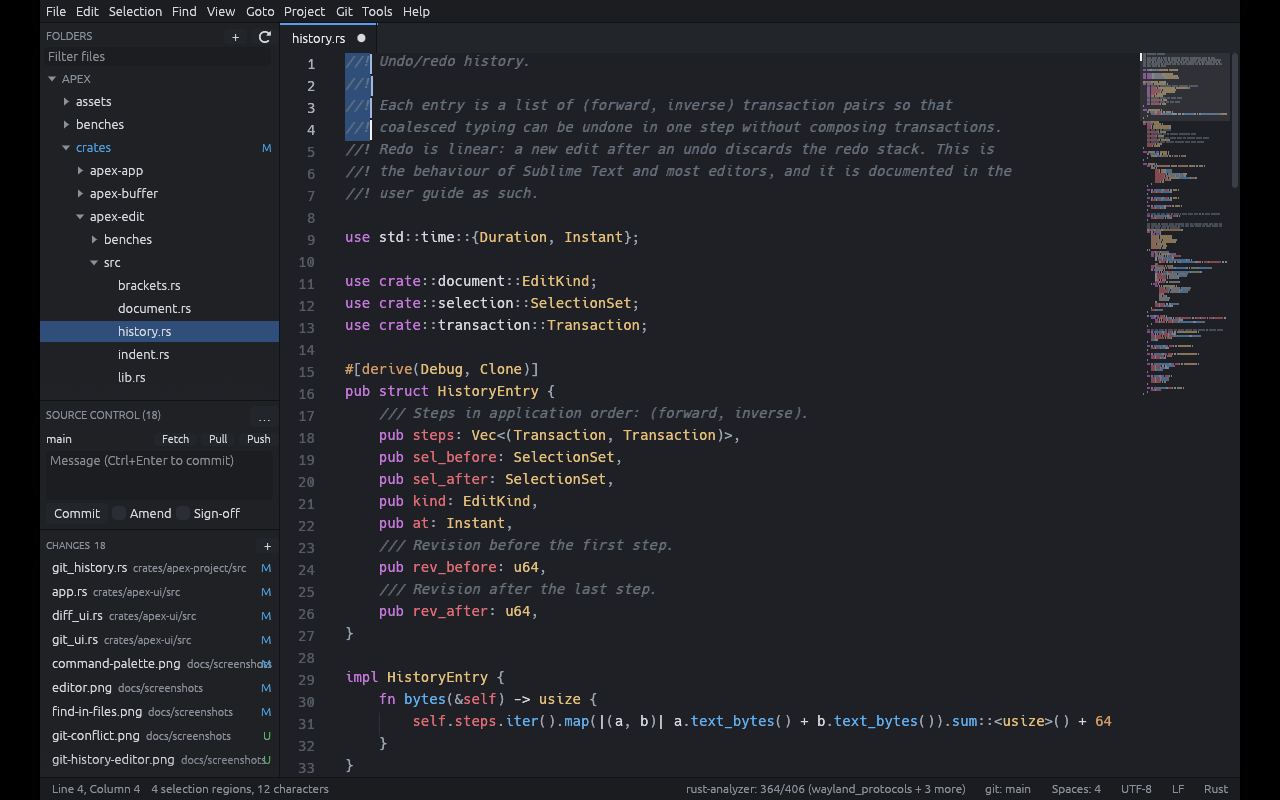
\includegraphics[width=0.9\textwidth]{multi-cursor.png}
\end{center}

\begin{longtable}{p{0.4\textwidth} p{0.54\textwidth}}
\toprule
\textbf{Keys} & \textbf{Action} \\
\midrule
\endhead
\key{Ctrl+Click} & Add a caret (or remove the one under the pointer). \\
\key{Ctrl+D} & Select the word under the caret, then add the next occurrence each press. \key{Ctrl+K Ctrl+D} skips one. \\
\key{Alt+F3} & Select every occurrence. \\
\key{Ctrl+Shift+L} & Split a selection into one caret per line. \\
\key{Alt+Shift+Up} / \key{Down} & Add a caret on the line above / below (the column is kept across short lines). \\
\key{Ctrl+Shift+Alt+Up} / \key{Down}, \key{Shift}+right-drag, middle-drag & Column selection. \\
\key{Ctrl+U} & Undo the last selection change. \\
\key{Escape} & Back to a single caret. \\
\key{Ctrl+L} & Select the line (repeat to extend). \\
\key{Ctrl+Shift+M} / \key{Ctrl+M} & Select inside brackets / jump to the matching bracket. \\
\key{Ctrl+Shift+J} & Select the indentation block. \\
\key{Ctrl+Shift+A} / \key{Ctrl+Shift+Alt+A} & Expand / shrink the selection by syntax scope. \\
\bottomrule
\end{longtable}

Pasting with as many clipboard lines as there are carets puts one line at
each caret. The status bar shows the caret count and selected characters.

\begin{tryit}
Put the caret on a variable name. Press \key{Ctrl+D} three times. Type a new
name. Press \key{Escape}. You have just renamed three occurrences in one
undo step.
\end{tryit}

\section{Bookmarks}

\key{Ctrl+F2} toggles a bookmark on the line; \key{F2} / \key{Shift+F2} jump
between bookmarks; \key{Ctrl+Shift+F2} clears them. Bookmarks move with the
text as you edit and are saved with the session.

\section{Snippets}

Type a trigger and press \key{Tab} (\texttt{fn} in Rust, \texttt{def} in
Python), or choose \menu{Edit > Insert Snippet}. \key{Tab} and
\key{Shift+Tab} move through the placeholders; \key{Escape} ends the
session. Your own snippets go in
\texttt{<config>/snippets/<language>.toml}:

\begin{Verbatim}
[[snippet]]
trigger = "log"
description = "Log a value"
body = "println!(\"${1:name} = {:?}\", ${1});$0"
\end{Verbatim}

Variables such as \texttt{\$FILENAME}, \texttt{\$SELECTION},
\texttt{\$CLIPBOARD} and \texttt{\$DATE}, and choices like
\texttt{\$\{1|a,b,c|\}}, follow the usual snippet syntax.

\section{Macros}

\menu{Tools > Macros}: \key{Ctrl+Alt+R} starts and stops recording,
\key{Ctrl+Alt+Shift+R} replays. A macro is a list of built-in commands and
typed text. It can be saved under a name and replayed from the command
palette. Macros cannot run programs or scripts.

\section{Spell checking}

\menu{Tools > Toggle Spell Check} (or \setting{spell\_check = true})
underlines misspelt words in prose files, and in comments and strings of
code. Right-click a word for suggestions, \menu{Add to dictionary} or
\menu{Ignore}. Dictionaries are Hunspell \texttt{.dic} word lists found in
the system locations or \texttt{<config>/dictionaries/<lang>.dic}; the
status bar says when none is found.

% ===========================================================================
\chapter{Navigation}

\begin{nutshell}
One box, \key{Ctrl+P}, finds files, lines, symbols and commands. Prefixes
choose which.
\end{nutshell}

\section{Goto Anything (\key{Ctrl+P})}

\begin{center}
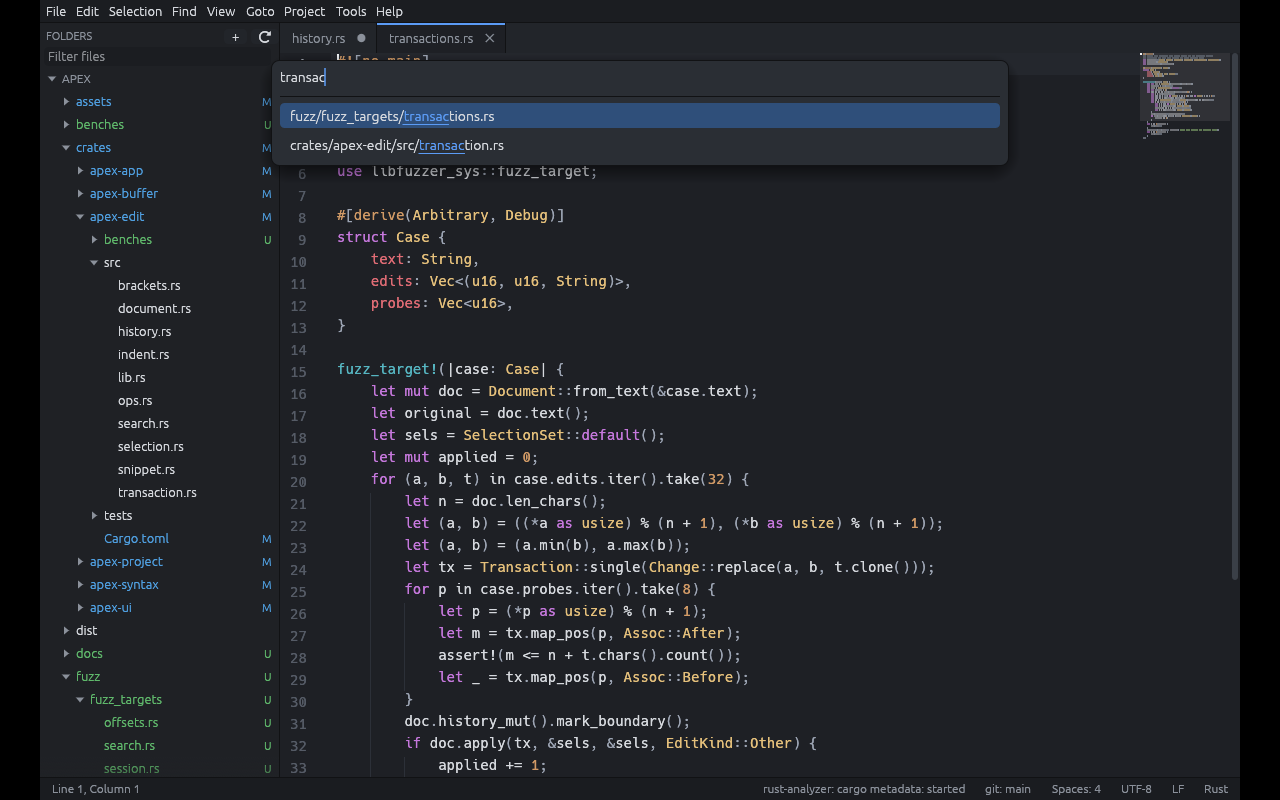
\includegraphics[width=0.9\textwidth]{goto-anything.png}
\end{center}

Type part of a file name or path to fuzzy-find it in the open folders. The
file is previewed as you move through the list; \key{Escape} takes you back
to where you were.

\begin{tabularx}{\textwidth}{l X}
\toprule
\textbf{Prefix} & \textbf{Finds} \\
\midrule
\texttt{:120} & Line 120 (\texttt{:120:8} for a column) in the current file \\
\texttt{@name} & Symbols in the current file (\key{Ctrl+R}) \\
\texttt{\#name} & Symbols across the project (\key{Ctrl+Shift+R}) \\
\texttt{>command} & Commands: the command palette (\key{Ctrl+Shift+P}) \\
\texttt{file@name}, \texttt{file:12} & A symbol or line in another file \\
\bottomrule
\end{tabularx}

\key{Ctrl+G} is a plain go-to-line dialog.

\section{Command palette (\key{Ctrl+Shift+P})}

\begin{center}
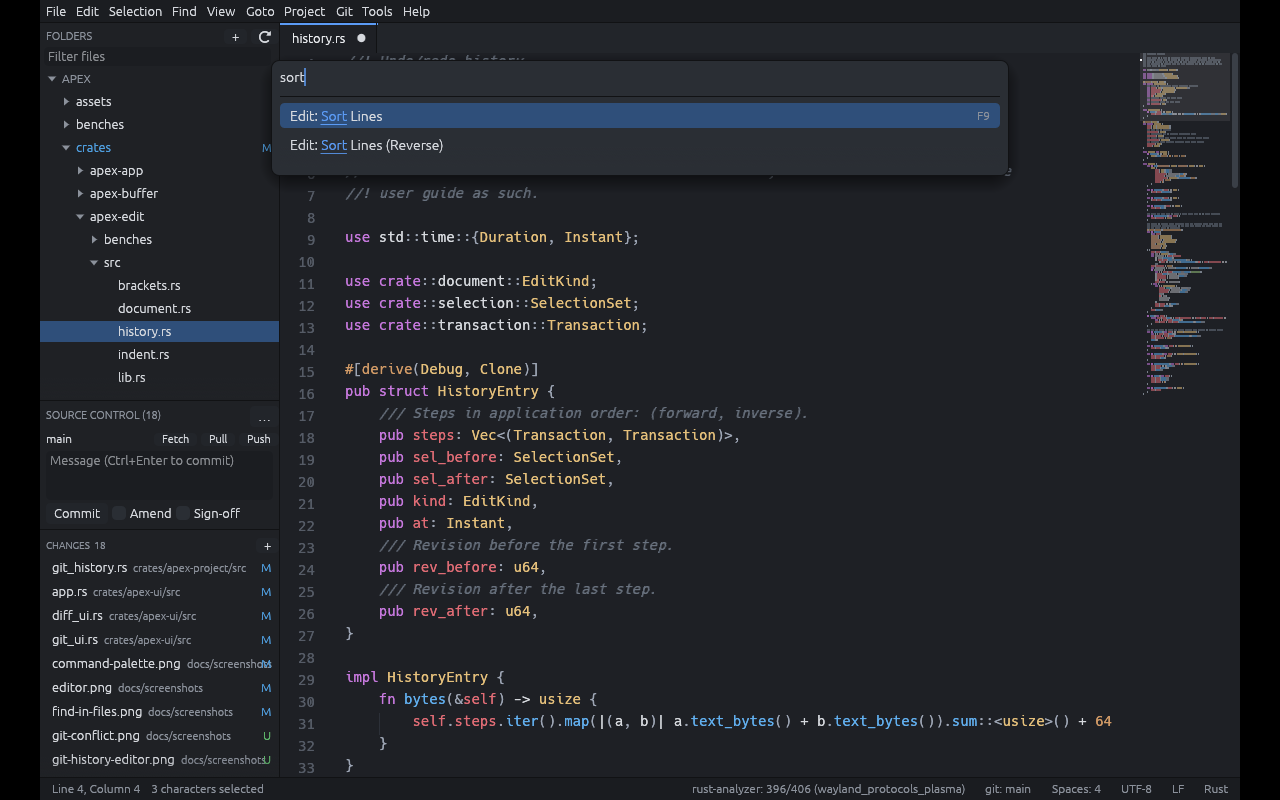
\includegraphics[width=0.9\textwidth]{command-palette.png}
\end{center}

Every command with its shortcut, fuzzy-filtered, most recent first.
Commands that take an argument prompt for it. Settings, themes, snippets,
macros, tasks and git status all have palette entries. Typing a command's
full name always picks that command, even when a recently used near-match
would otherwise rank higher.

\section{Moving around}

\begin{itemize}
\item \key{F12} go to definition, \key{Shift+F12} references (language
  server, or the project symbol index). \key{Alt+-} / \key{Alt+Shift+-} go
  back and forward through the jump history.
\item \key{Ctrl+M} jumps to the matching bracket; \key{Ctrl+Up} /
  \key{Ctrl+Down} scroll without moving the caret; \key{Ctrl+K Ctrl+C}
  centres the caret line.
\item \key{Ctrl+PgUp} / \key{Ctrl+PgDn} and \key{Ctrl+1} to \key{Ctrl+9}
  switch tabs; \key{Ctrl+Shift+T} reopens the last closed tab.
\item Folding: click the gutter arrows or use \key{Ctrl+Shift+[} /
  \key{Ctrl+Shift+]}, \key{Ctrl+K Ctrl+1} to \key{3} to fold to a level,
  \key{Ctrl+K Ctrl+J} to unfold all.
\item The minimap shows the whole file; click or drag it to scroll.
  Breadcrumbs above the editor show the enclosing symbols.
\end{itemize}

\section{Panes and tabs}

\key{Ctrl+\textbackslash} splits the pane. \menu{View > Layout} has single,
two and three columns, two rows and a grid (\key{Alt+Shift+1}, \key{2},
\key{3}, \key{8}, \key{5}). \key{Ctrl+K Ctrl+Left} / \key{Right} move focus
between panes. The same file can be open in several panes with independent
scroll positions and selections; edits show up everywhere at once.

Tabs: drag to reorder, right-click for close others / close to the right,
pin, copy path, reveal in the file manager. A file opened from the sidebar
with a single click is a \emph{preview} tab (italic title) that the next
preview replaces; editing it or double-clicking makes it permanent.

% ===========================================================================
\chapter{Search and replace}

\begin{nutshell}
\key{Ctrl+F} in the file, \key{Ctrl+Shift+F} across the project. Both
support regular expressions, whole word and case options.
\end{nutshell}

\section{In the file}

The find bar appears above the status bar. Matches are highlighted in the
text, the scrollbar and the minimap. \key{Enter} / \key{Shift+Enter} and
\key{F3} / \key{Shift+F3} step through matches; \key{Escape} returns to the
editor at the current match.

\begin{tabularx}{\textwidth}{l X}
\toprule
\textbf{Keys} & \textbf{Option} \\
\midrule
\key{Alt+R} & Regular expression (Rust \texttt{regex} syntax; errors show in the bar) \\
\key{Alt+C} & Case sensitive \\
\key{Alt+W} & Whole word \\
\key{Ctrl+E} & Use the selection as the search text \\
\key{Ctrl+F3} & Find the word under the caret \\
\menu{Find in Selection} & Restrict the search to the selected range \\
\bottomrule
\end{tabularx}

Replace (\key{Ctrl+H}) adds a replacement field: \key{Ctrl+Shift+H}
replaces the current match and moves on, \key{Ctrl+Alt+Enter} replaces all
in one undo step. Replacements support \texttt{\$1} and \texttt{\$\{name\}}
groups in regex mode and preserve case when the search is case-insensitive.
\menu{Find All} turns every match into a cursor.

\section{Across the project}

\begin{center}
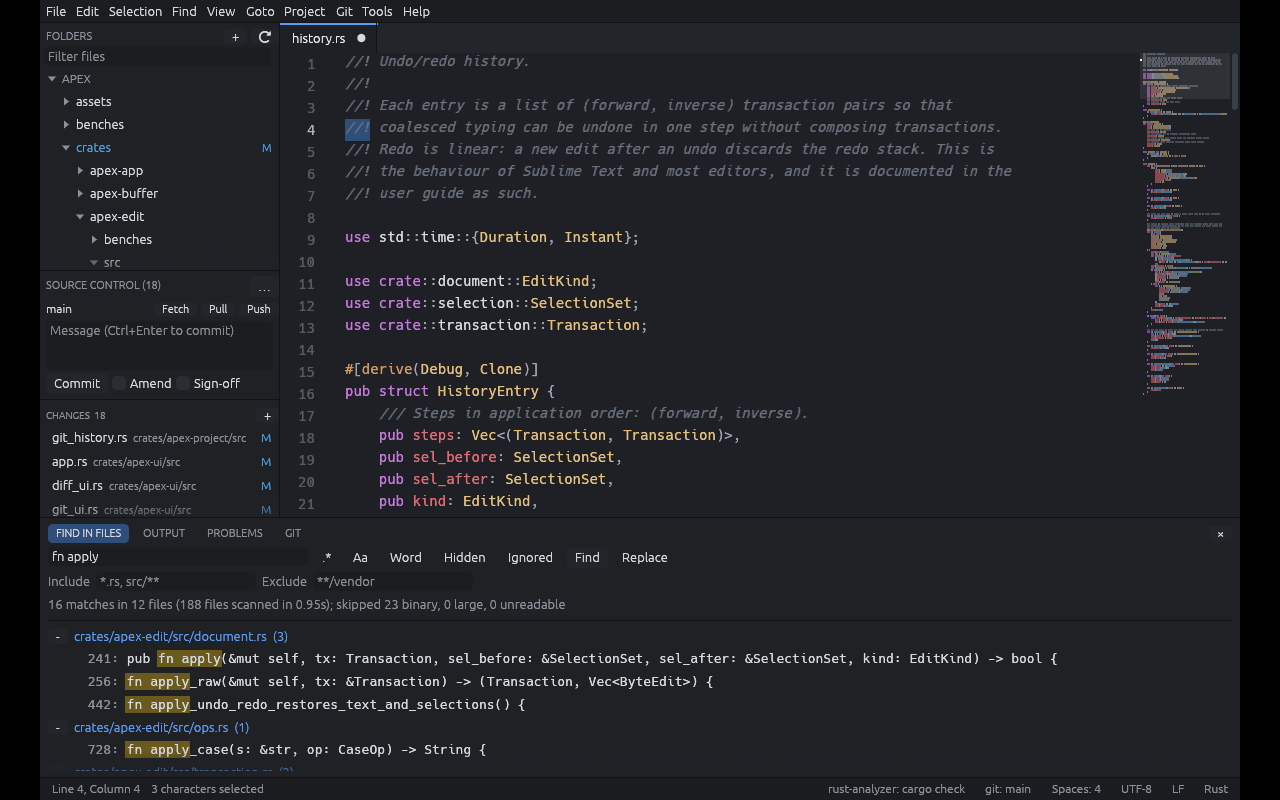
\includegraphics[width=0.9\textwidth]{find-in-files.png}
\end{center}

\menu{Find in Files} searches the open folders in the background with the
same syntax plus include and exclude globs (\texttt{*.rs, !target/**}).
Results are grouped by file with context lines; click one to open it at the
match. Binary files, \setting{exclude\_patterns} and \texttt{.gitignore}
entries are skipped.

\menu{Replace in Files} previews the count per file and asks first. Every
changed file is written atomically; files open in the editor are updated in
place and keep their undo history.

% ===========================================================================
\chapter{Projects, the sidebar and sessions}

\begin{nutshell}
Open folders, not projects. A project file is optional and only adds
settings and tasks. Everything you had open comes back next time.
\end{nutshell}

\section{Folders}

\menu{File > Open Folder} (\key{Ctrl+Shift+O}), dragging a folder onto the
window, \texttt{apex .} or the \menu{+} button in the sidebar add a folder
to the workspace. Several can be open at once. The sidebar reads only the
directories you expand, so a 100,000-file tree opens instantly; the index
behind Goto Anything and Find in Files is built in the background and kept
current by a file watcher.

Right-click an entry for new file, new folder, rename, duplicate, delete
(to the system bin, with confirmation), copy path, reveal, find in folder.
Files ignored by \texttt{.gitignore} and \setting{exclude\_patterns} are
dimmed or hidden. Git status is shown next to changed files.

\section{Remote files over SSH}\label{sec:remote}

\menu{File > Open Remote} opens a browser for a server. Type a host
(\texttt{user@server}, or an alias from \texttt{\textasciitilde/.ssh/config}),
press \textbf{Connect}, and click a file. Click a folder to go into it,
\textbf{Up} to go back. Apex runs your own \texttt{ssh}, so your keys,
agent, \texttt{ProxyJump} and the rest of your SSH config just work. The
server needs nothing but \texttt{sh}, \texttt{cat}, \texttt{ls} and
\texttt{cksum}.

\begin{itemize}
\item The tab is called \texttt{name (host)}.
\item \textbf{Save} writes back to the server. The file keeps its owner and
  permissions, and a dropped connection never leaves it half-written.
\item \textbf{Save As}, and \menu{File > Save to Remote} for any tab, pick
  a place in the same browser. It asks before replacing a file.
\item \textbf{Revert} takes the server's copy.
\item Every 5 seconds Apex checks each remote file. No unsaved edits: it
  reloads quietly. Unsaved edits: a note in the status bar; \textbf{Save}
  overwrites theirs, \textbf{Revert} takes theirs.
\end{itemize}

\subsection*{When the connection drops}

Nothing pops up. The tab title says \texttt{offline}. A save that fails
keeps your changes in the editor (and in crash recovery) and finishes by
itself when the server answers again, unless the file changed there in the
meantime; then you choose. Remote tabs do not come back after a restart.

\subsection*{Passwords and passphrases}

Keys and the agent are tried first. If a password or passphrase is needed,
a dialog asks, over the browser. Cancel or a wrong answer shows
``Permission denied''; press \textbf{Connect} to try again.

\begin{safenote}
Apex remembers the password so it does not ask again and so background
checks keep working. It is held \textbf{only in memory}, in pages locked so
they are never swapped to disk (and kept out of crash dumps on Linux). It is
never written to disk, the session, recovery or logs.

It is kept \textbf{while a file from that server is open or the browser
shows that server}. When the last one closes, the memory is overwritten with
zeros, released, and the shared SSH connection is closed. Quitting wipes it
too. A password the server rejects is forgotten at once. One-time codes are
never kept.

Background checks and automatic retries never ask; without a remembered
password they just show \texttt{offline}.

The text box you type into belongs to the GUI toolkit. Apex clears it when
the dialog closes but cannot promise no stray copy was left while you typed.
If that matters to you, use a key with an agent.
\end{safenote}

\begin{watchout}
The first connection to a new server records its host key without asking.
If a server's key later changes, Apex refuses to connect; check with the
server's owner, then fix \texttt{\textasciitilde/.ssh/known\_hosts}.
\end{watchout}

\section{Project files}

\menu{Project > Save Project As} opens a native Save panel and suggests
\texttt{<name>.apex-project}. Setting
\setting{native\_file\_dialogs = false} uses a path prompt instead.
The project file contains:

\begin{Verbatim}
# Apex project file. Safe to commit: it holds no session state.
folders = ["."]

[settings]
tab_width = 2

[[tasks]]
name = "Check"
command = ["cargo", "check"]
problem_matcher = "rustc"
\end{Verbatim}

Opening the project file restores the folders and applies the
\texttt{[settings]} overrides on top of your own. Tasks from a project file
run only after you trust the workspace (chapter~\ref{ch:tasks}).

\section{Sessions and recovery}

When you quit, the open folders, tabs, selections, scroll positions, pane
layout, bookmarks and window size are saved and restored on the next start.
Unsaved buffers are kept too.

Every few seconds unsaved changes are snapshotted to the data directory.
After a crash or power cut the next start offers to restore them.

\begin{safenote}
Files changed on disk by another program are noticed (on focus and every
two seconds). An unmodified buffer reloads silently; a modified one asks
whether to reload or keep your version. Saving over a file that changed
since it was loaded asks first. Apex never silently overwrites someone
else's edit.
\end{safenote}

% ===========================================================================
\chapter{Configuration}

\begin{nutshell}
\key{Ctrl+,} opens a searchable settings panel. Everything is plain TOML in
the configuration directory. There is no scripting; the editor only ever
reads these files.
\end{nutshell}

\begin{center}
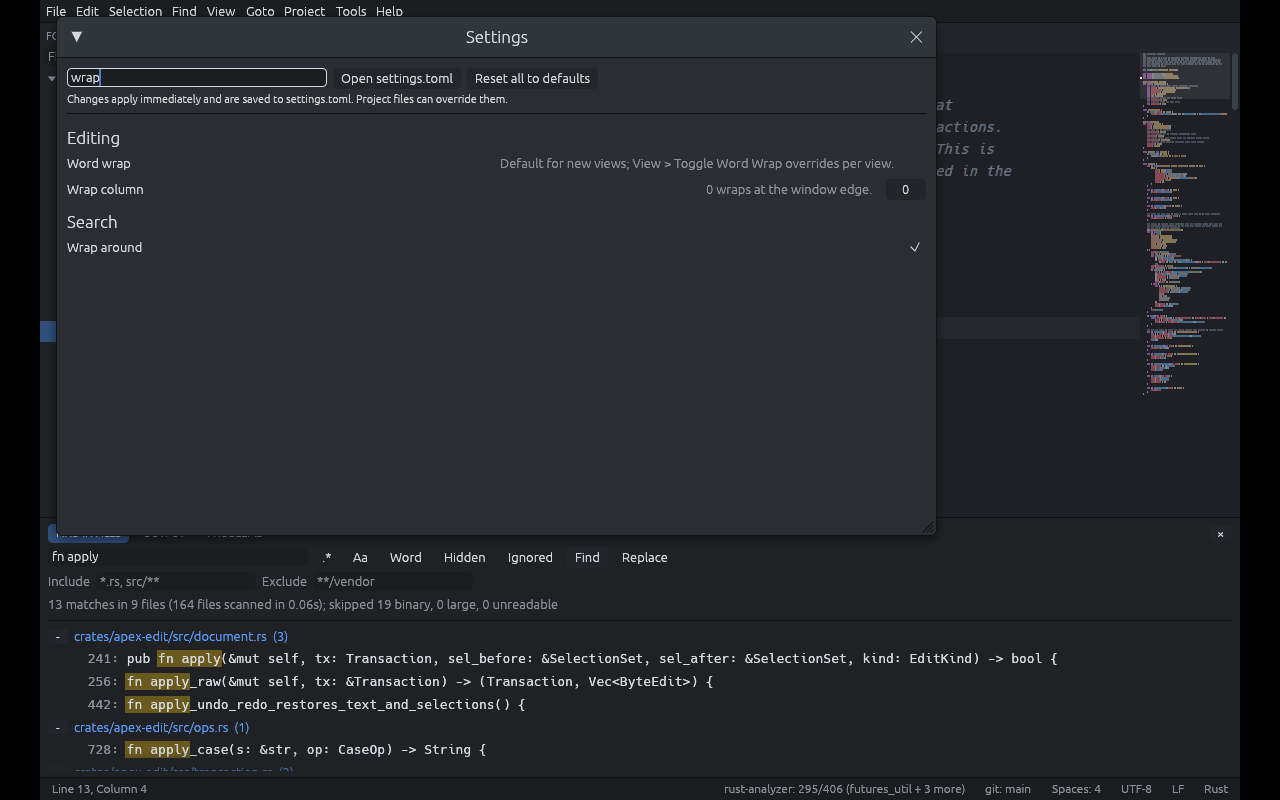
\includegraphics[width=0.9\textwidth]{settings.png}
\end{center}

\section{Settings}

Changes apply immediately and are written to \texttt{settings.toml}, which
stores only the keys you changed. \menu{Open settings.toml} edits the file
directly; saving it reloads the settings, and problems (unknown keys, wrong
types, out-of-range values) are reported in a dialog rather than ignored.

Layers, lowest first: built-in defaults, \texttt{settings.toml}, the
\texttt{[settings]} table of the open project file.

Open, folder selection and Save As use native system dialogs by default,
including Open Project and Save Project As. Set
\setting{native\_file\_dialogs = false} to use the in-app path prompt instead.

\begin{Verbatim}
theme = "Apex Light"
font_family = "JetBrains Mono"
font_size = 15
tab_width = 2
word_wrap = true
rulers = [80, 120]
trim_trailing_whitespace_on_save = true
vim_mode = true
spell_check = true
spell_language = "en_GB"
native_file_dialogs = true      # false: an in-app path prompt with Tab completion
exclude_patterns = ["target", "node_modules", "*.min.js"]

[lsp_servers]
rust = ["rust-analyzer"]
python = ["pyright-langserver", "--stdio"]
\end{Verbatim}

\section{Key bindings}

\menu{Tools > Open Keymap File} creates \texttt{<config>/keymap.toml}, merged
on top of the defaults:

\begin{Verbatim}
[[bindings]]
keys = "primary+k primary+t"      # chords are space-separated
command = "edit.title_case"
context = "editor"                # global, editor, find, overlay, sidebar

[[bindings]]
keys = "f5"
command = "build.run"
arg = "Cargo: test"               # optional command argument

[[macos]]                         # platform sections: [[linux]], [[windows]], [[macos]]
keys = "primary+shift+f"
command = "find.in_files"
\end{Verbatim}

\texttt{primary} is \key{Ctrl} on Linux and Windows and \key{Cmd} on macOS.
\menu{Tools > Keyboard Shortcuts} lists the effective bindings and reports
conflicts; the status bar shows a pending chord.

\section{Themes}

Eight themes are built in. \menu{View > Theme} switches, and
\setting{theme\_mode = "auto"} follows the system's dark or light setting.
User themes are TOML files in \texttt{<config>/themes/}:

\begin{Verbatim}
name = "My Theme"
dark = true

[ui]
background = "#1e2127"
text = "#d7dae0"
accent = "#61afef"

[editor]
background = "#1e2127"
caret = "#528bff"
selection = "#3e4451"

[syntax]
keyword = { fg = "#c678dd", bold = false }
string = { fg = "#98c379" }
comment = { fg = "#5c6370", italic = true }
\end{Verbatim}

Unknown keys are reported; missing keys fall back to the base theme.

\section{Dictionaries}

Hunspell \texttt{.dic} word lists are looked up in:
\begin{itemize}
\item \texttt{/usr/share/hunspell} and \texttt{/usr/share/myspell}
\item \texttt{\textasciitilde/Library/Spelling} (macOS)
\item \texttt{<config>/dictionaries/}
\item \texttt{/usr/share/dict/words}
\end{itemize}
Words you add go to \texttt{<config>/dictionaries/user.txt}.

% ===========================================================================
\chapter{Git}
\label{ch:git}

\begin{nutshell}
Apex reads your repository on its own and runs \emph{your} installed
\texttt{git} for anything that changes it. The Source Control panel in the
sidebar does staging and commits; the Git menu has everything else:
diffs, blame, branches, log, stash, conflicts, push and pull, GitHub pull
requests and commit-history editing.
\end{nutshell}

\begin{safenote}
Apex stores no git credentials or tokens. Push and pull use your credential
helper and SSH agent. When git or ssh asks for a password or passphrase,
Apex shows a dialog, hands the answer to git once, and forgets it. GitHub
features use the GitHub CLI (\texttt{gh}), which holds your login. Commands
that run \texttt{git} ask you to \textbf{trust the folder} first, because
git runs the repository's hooks.
\end{safenote}

\section{What you see without doing anything}

\begin{itemize}
\item \textbf{Gutter marks} beside the line numbers show added, modified and
  deleted lines against the index. They update as you type and the minimap
  shows them too. \setting{git\_gutter = false} turns them off.
\item \textbf{Status bar}: the branch (or a short commit id when detached),
  commits to push and pull, the branch's pull request, and any merge or
  rebase in progress.
\item \textbf{Folder tree}: changed, added, untracked and conflicted files
  are marked.
\end{itemize}

\menu{Goto > Next Change} / \menu{Previous Change} jump between hunks.
\menu{Revert Change} restores the hunk under the caret after confirming, as
an undoable edit. \menu{Compare with Saved / Index / HEAD} opens a
side-by-side diff. \menu{File History} lists the commits that touched the
file; choosing one shows it.

\section{The Source Control panel}

\begin{center}
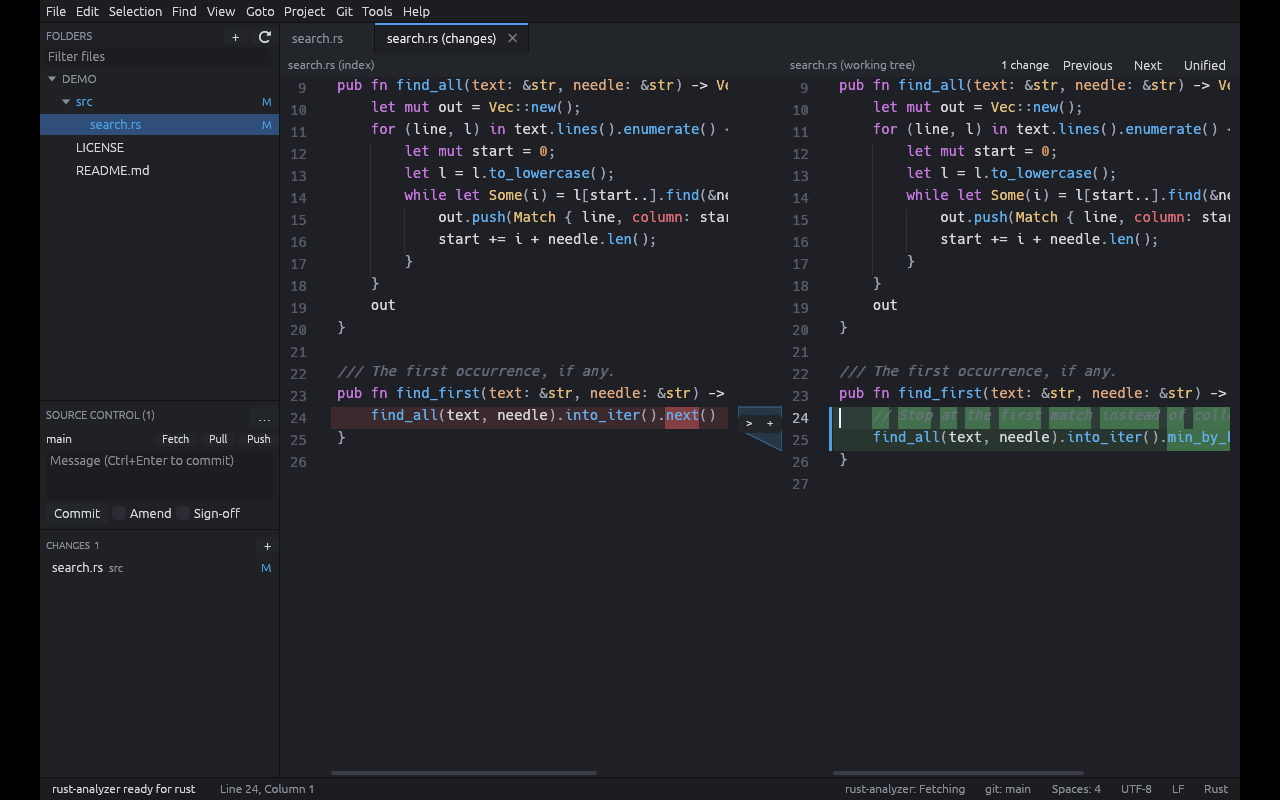
\includegraphics[width=0.95\textwidth]{git-side-by-side.png}
\end{center}

The lower half of the sidebar shows the repository of the active file: the
branch and how far it is ahead of or behind its upstream, the commit box,
and changed files grouped as \menu{Merge conflicts}, \menu{Staged changes}
and \menu{Changes}. Drag the divider to resize it; \setting{git\_sidebar =
false} or \menu{Git > Toggle Source Control Panel} hides it.

\begin{itemize}
\item Click a file to preview it, double-click to open its changes. Hover a
  file for \menu{+} stage, \menu{--} unstage and discard; right-click for the
  full list.
\item \menu{Commit} (or \key{Ctrl+Enter} in the message box) commits the
  staged changes. With nothing staged it offers to commit all tracked
  changes. \key{Up} and \key{Down} in an empty box recall earlier messages;
  the number beside Sign-off is the summary line's length (50 recommended,
  72 at most).
\item \menu{Amend} rewrites the last commit; \menu{Sign-off} adds a
  \texttt{Signed-off-by} trailer.
\item \menu{Undo Last Commit} removes the last commit after confirming,
  keeps its changes staged and puts its message back in the box.
\item Your hooks run as usual; their output is in the GIT tab.
\end{itemize}

\begin{tryit}
Edit a file in a repository. Click \menu{+} next to it in the Source Control
panel. Type a message, press \key{Ctrl+Enter}. Open \menu{Git > Show Log}
and see your commit at the top.
\end{tryit}

\section{Side-by-side diffs}

\menu{Open Changes} (double-click a file in the panel), \menu{Open Staged
Changes}, the Compare commands and \texttt{apex --diff old new} show the two
versions next to each other.

\begin{itemize}
\item Both sides have syntax colours. Removed lines are tinted on the left,
  added lines on the right, changed words more strongly. A strip between the
  sides links each change.
\item When the right side is your file, it is the real document: edit, undo
  and save there as usual.
\item The strip's buttons act on one change: \menu{>} replaces it with the
  left side (undoable), \menu{+} stages it, \menu{--} unstages it.
\item Long unchanged stretches are folded on both sides, keeping three lines
  of context; \menu{Expand / Collapse} in the header toggles this.
\item \menu{Next / Previous} jump between changes; \menu{Unified} shows the
  same comparison as a unified diff. Closing the tab closes both sides.
\end{itemize}

\section{Staging}

\begin{itemize}
\item \menu{Stage File / Unstage File} for the active file; \menu{Stage All
  Changes / Unstage All Changes} for the repository.
\item \menu{Stage Change at Caret} stages just the hunk under the caret;
  \menu{Stage Selected Lines} stages only the changed lines your selections
  touch (several cursors work). Save first: staging uses the file on disk.
\item \menu{Discard File Changes} restores the file from the index after
  confirming; for an untracked file it offers to delete it.
\end{itemize}

\section{Fetch, pull and push}

Apex only talks to the network when you ask, or when
\setting{git\_auto\_fetch\_minutes} is above 0.

\begin{itemize}
\item \menu{Fetch} fetches every remote and prunes deleted branches.
\item \menu{Pull} follows \setting{git\_pull\_mode}: \texttt{ff-only}
  (default) refuses to create a merge commit, \texttt{rebase} replays your
  commits, \texttt{merge} merges.
\item \menu{Push} pushes to the upstream branch. A branch without one is
  published to \texttt{origin} after asking.
\item \menu{Sync} pulls then pushes. \menu{Force Push (with Lease)} replaces
  the upstream branch after confirming and refuses if the remote changed
  since your last fetch.
\item Progress appears in the status bar; \menu{Cancel Git Command} stops a
  slow transfer.
\end{itemize}

\section{GitHub and other code hosts}

\menu{Git > Remote} builds links from the repository's remote (GitHub,
GitLab, Bitbucket, Codeberg and Gitea) and opens them in your browser:
\menu{Open File on Remote}, \menu{Copy Permalink} (with the selected lines),
\menu{Open Commit / Branch on Remote}, \menu{Compare Branch on Remote}. Apex
makes no network request for these.

\menu{Git > GitHub} uses the GitHub CLI. Install it and run \texttt{gh auth
login} once.

\begin{itemize}
\item \menu{Create Pull Request}: title and description filled in from the
  branch's commits, base branch, draft. Unpushed commits are pushed first.
\item The status bar shows the branch's pull request, its checks and review
  state. It refreshes after you push or create a pull request, and on
  \menu{Refresh Pull Request Status}; Apex does not poll GitHub.
\item \menu{Pull Requests} lists open ones to check out, show the diff or
  open in the browser. \menu{Pull Request Checks} lists the checks.
\end{itemize}

\section{Branches, log and stash}

\begin{center}
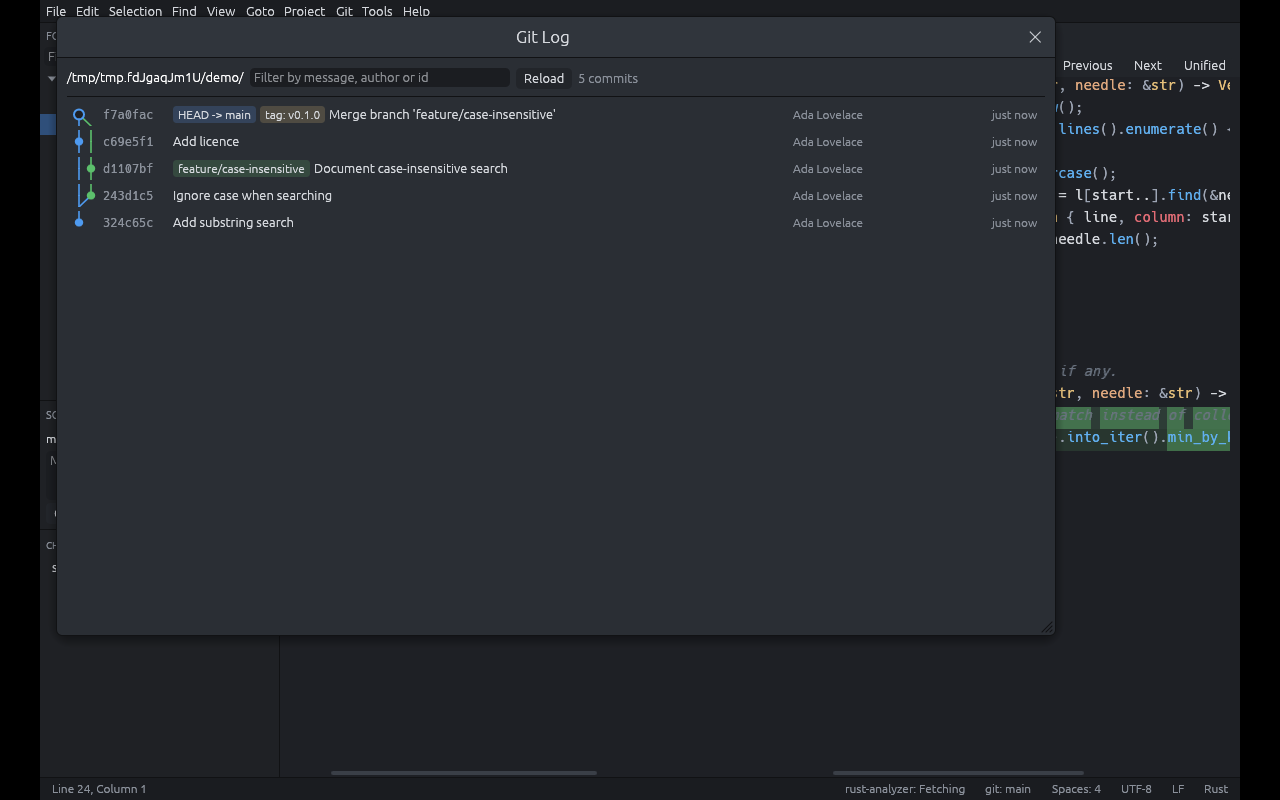
\includegraphics[width=0.9\textwidth]{git-log.png}
\end{center}

\begin{itemize}
\item \menu{Switch Branch} (or click the branch name in the panel) lists
  local branches and remote ones without a local copy; the first entry
  creates a new branch. Git refuses to switch when your changes would be
  overwritten: stash them first.
\item \menu{Create / Rename / Delete Branch} and \menu{Merge Branch into
  Current} are under \menu{Git > Branches}. Deleting refuses a branch with
  unmerged commits.
\item \menu{Show Log} opens every commit of every branch and tag with a lane
  graph. Type to filter; \key{Enter} shows a commit; right-click to copy its
  id, create a branch there, check it out, cherry-pick it, revert it, or
  open it on the remote.
\item \menu{Line History of Selection} shows how the selected lines changed
  over time.
\item \menu{Stash Changes} stashes everything including untracked files;
  \menu{Stashes} lists them with Apply, Pop, Show and Drop.
\end{itemize}

\section{Merge conflicts}

\begin{center}
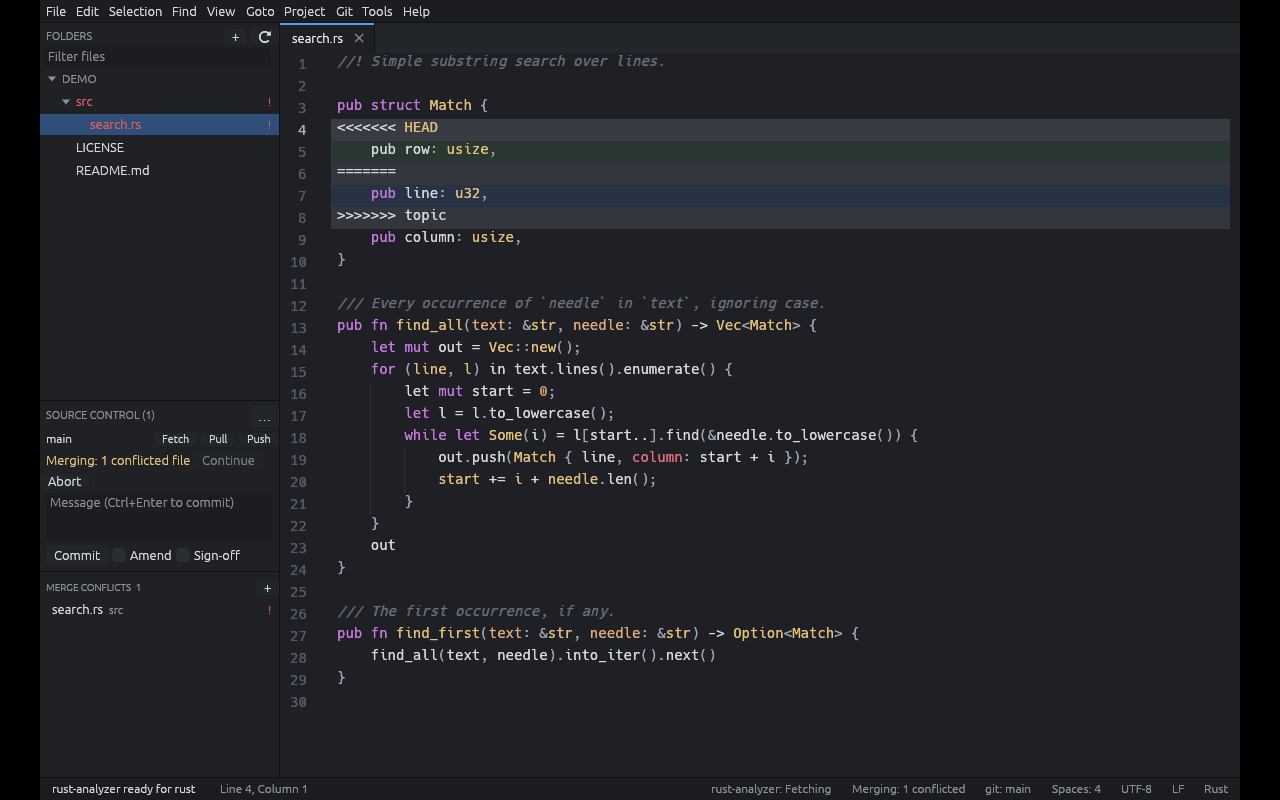
\includegraphics[width=0.9\textwidth]{git-conflict.png}
\end{center}

When a merge, rebase, cherry-pick or revert stops on conflicts, the status
bar and the panel say so, and the conflicted files are listed under
\menu{Merge conflicts}.

\begin{enumerate}
\item Conflict blocks are tinted: ours, theirs and the marker lines differ.
  \menu{Next / Previous Conflict} move between them.
\item With the caret in a block, \menu{Accept Current Change}, \menu{Accept
  Incoming Change} or \menu{Accept Both Changes} (\menu{Git > Conflicts} or
  right-click) replace the block. Each is an ordinary undoable edit.
\item Save, then \menu{Mark Resolved} to stage the file (it warns if markers
  are left).
\item When nothing is conflicted, \menu{Continue} in the panel finishes the
  merge or moves the rebase on. \menu{Abort} returns to where you started,
  after confirming.
\end{enumerate}

\section{Blame}

\menu{Git > Toggle Blame} (\key{Ctrl+K Ctrl+G}) adds a gutter column with
the author and age of the commit that last changed each line, shaded so
newer changes stand out. Unsaved edits show as \emph{Not committed}. Hover
for the full message; click to open the commit in a read-only tab.
\setting{git\_blame\_inline = true} also writes it after the caret line.

\section{Edit Commit History}

\begin{center}
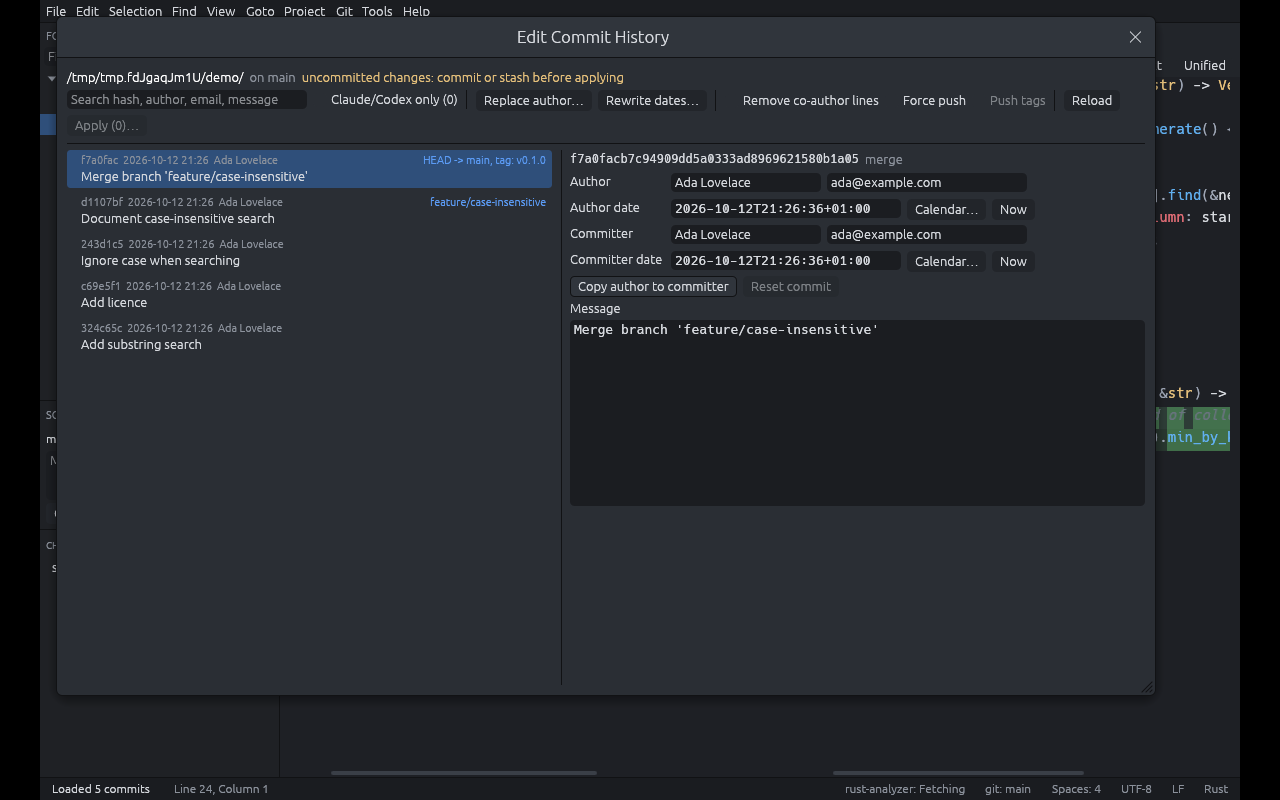
\includegraphics[width=0.9\textwidth]{git-history-editor.png}
\end{center}

\menu{Git > Edit Commit History} opens an editor for the metadata of every
commit in the repository, newest first. Nothing changes until you apply.

\begin{itemize}
\item Select a commit to edit its author and committer (name, email, date)
  and its message. \menu{Calendar} picks a day and time; \menu{Now} sets the
  current time. \menu{Reset commit} undoes the edits to one commit.
\item Search filters by hash, author, email or message. \menu{Claude/Codex
  only} lists commits that mention Claude, Codex or Anthropic.
\item \menu{Replace author} sets a new author on every matching commit.
  \menu{Rewrite dates} gives every commit a random time inside a daily
  window across a range of days, keeping their order. \menu{Remove co-author
  lines} drops \texttt{Co-authored-by:} trailers and AI attribution blocks.
\item \menu{Apply} lists the commits that will change and asks first. The
  repository must be clean. Apex tags the current HEAD as
  \texttt{apex-backup-<time>}, rewrites local branches and tags with
  \texttt{git filter-branch}, then cleans up. To go back:
  \texttt{git reset --hard apex-backup-<time>}.
\item \menu{Force push} then pushes every branch with
  \texttt{--force-with-lease}; you must type \texttt{FORCE} to confirm.
\end{itemize}

\begin{watchout}
Rewriting history gives every changed commit, and every commit after it, a
new hash. Anyone who has the old history must re-clone or reset. Try it on
a throwaway clone first, and coordinate with anyone else using the
repository.
\end{watchout}

\section{The GIT output tab}

Every command Apex runs, with its output, is shown in the \menu{GIT} tab of
the bottom panel (\menu{Git > Show Git Output}). Commands run one at a time
in the background; \menu{Git > Cancel Git Command} stops the running one.
Git never prompts on a terminal.

% ===========================================================================
\chapter{Build tasks}
\label{ch:tasks}

\begin{nutshell}
\key{Ctrl+B} runs the build for the folder; \key{Ctrl+Shift+B} picks a
task. Errors land in the Problems tab and are underlined in the editor.
\end{nutshell}

Output streams into the bottom panel; \key{Escape} or \menu{Cancel Build}
stops the process and its children.

\section{Where tasks come from}

\begin{itemize}
\item \textbf{Detected}: \texttt{Cargo.toml} gives cargo build, test, run,
  clippy and check; \texttt{go.mod}, \texttt{package.json},
  \texttt{Makefile}, \texttt{CMakeLists.txt} and Python project files give
  their usual tasks. Single files get ``run file'' tasks for Python, Rust,
  shell, JavaScript, Go and Lua.
\item \textbf{Project file} \texttt{[[tasks]]} entries:
\end{itemize}

\begin{Verbatim}
[[tasks]]
name = "Test (verbose)"
command = ["cargo", "test", "--", "--nocapture"]
cwd = "crates/apex-edit"          # relative to the workspace root
env = { RUST_BACKTRACE = "1" }
shell = false                     # true runs command[0] through sh -c / cmd /C
timeout_secs = 600                # 0 = no limit
problem_matcher = "rustc"         # rustc, gcc, go, python, generic, or a regex
\end{Verbatim}

A custom matcher is a regular expression with named groups \texttt{file},
\texttt{line}, optional \texttt{col} and \texttt{message}.

\section{Trust}

\begin{safenote}
Tasks from a project file can run any program, so they are disabled until
you trust the workspace: the first attempt shows the command and asks.
\menu{Project > Trust Workspace} manages the decision, which is remembered
per folder in your data directory and never inside the repository. The
first line of the Output panel is always the exact command and directory
used. Commands never go through a shell unless \texttt{shell = true}, and
output is stripped of terminal escape sequences before it is shown. A task
inherits Apex's environment, as a command typed in a terminal would.
\end{safenote}

\section{Problems}

Matched errors and warnings appear in the \menu{Problems} tab with file,
line and message; click one to jump there. Language-server diagnostics
share the same list. The status bar shows the count.

% ===========================================================================
\chapter{Language servers}

\begin{nutshell}
Optional. If a known server is on your PATH and the folder is trusted, it
starts when you open a file of its language and gives you completion,
diagnostics, hover, go to definition, rename and formatting. Everything
else works without one.
\end{nutshell}

\begin{safenote}
Servers act on the whole folder, and some run its code: rust-analyzer runs
a Rust project's build scripts. So a server starts only in a folder you
have trusted (\menu{Project > Trust Workspace}). In an untrusted folder the
status bar says the server was not started; trust the folder and it
starts at once.
\end{safenote}

\section{Starting a server}

With \setting{lsp\_enabled = true} (the default) a known server starts the
first time you open a file of its language, if it is on your PATH:

\begin{tabularx}{\textwidth}{l X}
\toprule
\textbf{Language} & \textbf{Server} \\
\midrule
Rust & \texttt{rust-analyzer} \\
Python & \texttt{pyright-langserver}, \texttt{pylsp} \\
TypeScript, JavaScript & \texttt{typescript-language-server} \\
Go & \texttt{gopls} \\
C, C++ & \texttt{clangd} \\
Lua, Bash & \texttt{lua-language-server}, \texttt{bash-language-server} \\
JSON, CSS, HTML & the \texttt{vscode-*-language-server} packages \\
YAML, Markdown, TOML & \texttt{yaml-language-server}, \texttt{marksman}, \texttt{taplo} \\
Java, Kotlin, Swift & \texttt{jdtls}, \texttt{kotlin-language-server}, \texttt{sourcekit-lsp} \\
PHP, Ruby, C\# & \texttt{intelephense}, \texttt{solargraph}, \texttt{omnisharp} \\
\bottomrule
\end{tabularx}

Other servers, or different commands, go in settings:

\begin{Verbatim}
[lsp_servers]
zig = ["zls"]
python = ["ruff", "server"]
\end{Verbatim}

The status bar shows the server's state and progress. \menu{Tools > Restart
Language Server} restarts it; a server that exits three times in a row is
left stopped and its last stderr lines are shown.

\section{What you get}

\begin{itemize}
\item Diagnostics underlined and listed in Problems; hover shows the
  message.
\item Completion merged with word and snippet completions.
\item Hover documentation and signature help.
\item \key{F12} definition, \key{Shift+F12} references, document and
  workspace symbols in Goto Anything.
\item \menu{Rename Symbol} (\key{F7}), \menu{Code Actions}
  (\key{Ctrl+K Ctrl+I}), \menu{Format Document} (\key{Ctrl+Shift+I}, also
  \setting{format\_on\_save}). Edits to files not open in the editor are
  previewed and confirmed first.
\end{itemize}

Servers run as child processes with only the workspace folders as roots.
The client makes no network connections.

% ===========================================================================
\chapter{Vim mode}

\begin{nutshell}
A modal layer over Apex's own editing model: normal, insert, visual and
visual-line modes, operators, text objects, registers, the dot command and
\texttt{:} commands. Not a full Vim; what is listed here is what works.
\end{nutshell}

\begin{center}
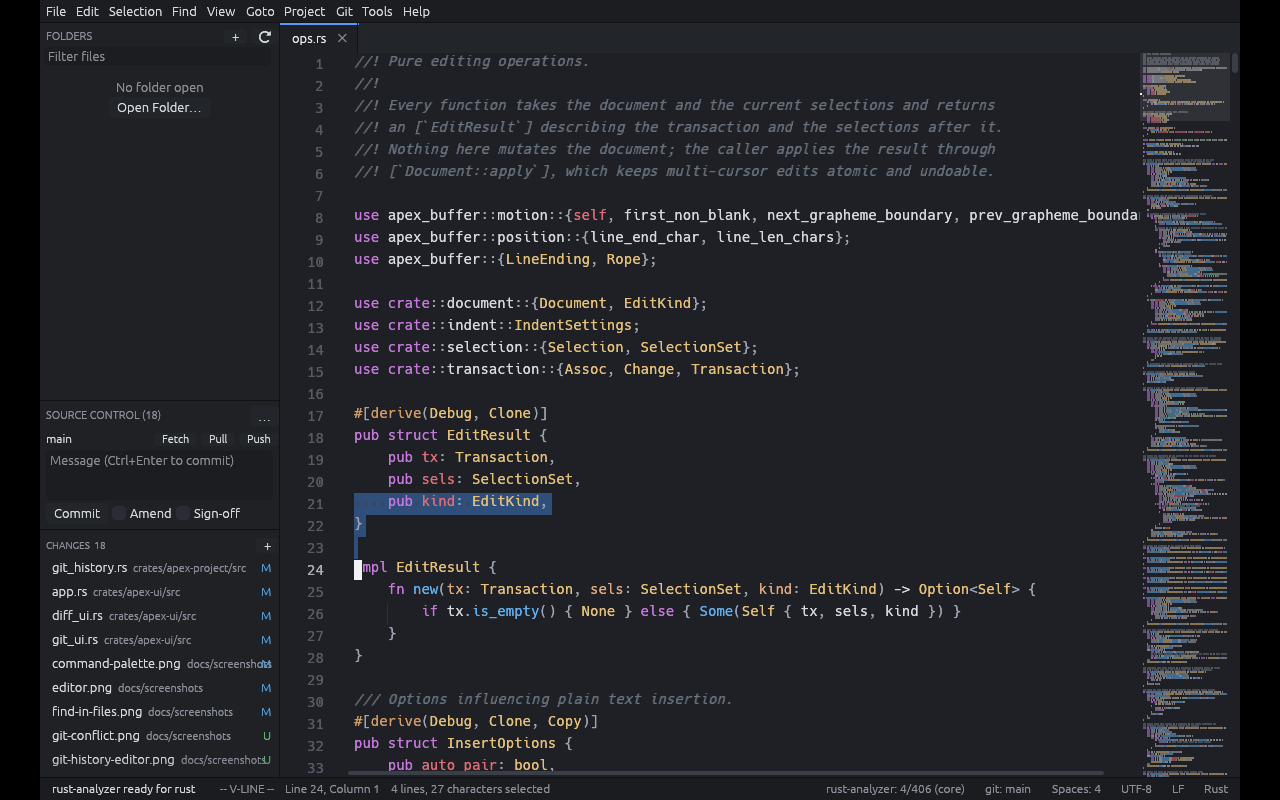
\includegraphics[width=0.9\textwidth]{vim-mode.png}
\end{center}

Turn it on with \setting{vim\_mode = true}, or for the session with
\menu{Tools > Toggle Vim Mode}. The status bar shows the mode, partially
typed keys, and the command line. The mouse, menus, the palette, Find and
all \key{Ctrl} shortcuts keep working.

\section{Modes and motions}

\key{i} \key{a} \key{I} \key{A} \key{o} \key{O} enter insert mode;
\key{Esc} returns (the insert session is one undo step). \key{v} and
\key{V} are visual and visual-line; \key{o} swaps the ends. \key{:} opens
the command line; \key{/} and \key{?} search.

Motions: \texttt{h j k l}, arrows, \texttt{0 \^{} \$ |}, \texttt{w W b B e E
ge}, \texttt{gg G}, \texttt{\{ \}}, \texttt{\%}, \texttt{f F t T ; ,},
\texttt{H M L}, \key{Ctrl+F} \key{Ctrl+B} \key{Ctrl+D} \key{Ctrl+U},
\texttt{n N * \#}, marks with \texttt{m} and \texttt{'}. Counts work with
every motion.

\section{Operators and text objects}

\texttt{d c y > < = gu gU g\textasciitilde}, each with a motion or text
object, doubled for whole lines (\texttt{dd}, \texttt{3dd}), and on the
selection in visual mode. Shortcuts: \texttt{x X s S D C Y J r
\textasciitilde\ p P}; \texttt{R} is replace mode.

Text objects: \texttt{iw aw iW aW ip ap is as}, brackets \texttt{( \{ [ <},
quotes \texttt{" ' `}, and tags \texttt{it at}.

\section{Registers, repeat, command line}

\texttt{"a} to \texttt{"z} named (capitals append), \texttt{"0} last yank,
\texttt{"1} to \texttt{"9} deletes, \texttt{"\_} black hole, \texttt{"+}
and \texttt{"*} the system clipboard. \texttt{.} repeats the last change;
\texttt{u} undoes, \key{Ctrl+R} redoes.

\texttt{:w}, \texttt{:q}, \texttt{:wq}, \texttt{:x}, \texttt{:e file},
\texttt{:N}, \texttt{:s/pat/rep/g}, \texttt{:\%s/.../.../g}, \texttt{:noh},
\texttt{:set wrap|nu|rnu|spell}, \texttt{:sp}, \texttt{:vs}, \texttt{:bn},
\texttt{:bp}, \texttt{:reg}. \texttt{:q} closes the tab; \texttt{:qa} quits.

\begin{watchout}
No visual block mode (use column selection), no \texttt{q} macros (use the
editor's recorder), no \texttt{:g}, mappings or \texttt{.vimrc}.
\end{watchout}

% ===========================================================================
\chapter{Troubleshooting}

\begin{nutshell}
Most problems are one of these. Each entry is a symptom followed by the
thing to try.
\end{nutshell}

\begin{description}[style=nextline]
\item[Where are the logs?] Apex logs to stderr. Run \texttt{apex --log
  debug} from a terminal. There is no telemetry and no log file unless you
  redirect one.
\item[The window is blank or does not open.] Try OpenGL with
  \texttt{WGPU\_BACKEND=gl}, or \texttt{WGPU\_BACKEND=vulkan} with a
  software Vulkan driver on machines without a GPU. On Wayland without
  decorations, \texttt{WINIT\_UNIX\_BACKEND=x11} forces X11.
\item[A settings dialog on start-up.] It lists keys in
  \texttt{settings.toml} or the project file that were unknown or out of
  range; those were ignored and everything else applied.
\item[``No dictionary found''.] Install a Hunspell dictionary
  (\texttt{hunspell-en-gb} on Debian and Ubuntu) or put a word list at
  \texttt{<config>/dictionaries/<lang>.dic}.
\item[A language server does not start.] Check its program is on the PATH
  of the shell that launched Apex; desktop launchers often have a shorter
  PATH. Configure the full path under \texttt{[lsp\_servers]}.
\item[A build task is greyed out.] Tasks from a project file run only after
  \menu{Project > Trust Workspace}.
\item[The Open or Save As dialog does not appear (macOS).] If the system
  reports a panel failure, Apex opens a path prompt instead. Enter the
  file or folder path; \key{Tab} completes it. Cancelling keeps your
  unsaved work. Set \setting{native\_file\_dialogs = false} to use the path
  prompt immediately for every request. A stalled macOS panel service can
  still block the system dialog. If file dialogs also hang in other
  applications, preserve unsaved work and restart macOS.
\item[Fonts show boxes.] Set \setting{font\_family} to an installed font
  with the glyphs you need.
\item[Keys do nothing in the editor.] Vim mode may be on (the status bar
  says \texttt{-- NORMAL --}): press \key{i} to insert or turn it off under
  \menu{Tools}. A pending chord such as \key{Ctrl+K} is shown in the status
  bar; \key{Escape} cancels it.
\item[Recovering work after a crash.] Start Apex; it offers the snapshots
  it kept. They live in the data directory under \texttt{recovery/}.
\item[Resetting everything.] Delete the configuration and data directories
  listed in \menu{Help > About}.
\item[Reporting a problem.] Include the version (\texttt{apex --version}),
  the platform, the \texttt{--log debug} output around the problem and, for
  crashes, the \texttt{RUST\_BACKTRACE=1} output. Nothing is sent
  automatically.
\end{description}

\end{document}
